\chapter{SYSTEM DESIGN }

 \section{Use case model}
\begin{figure}[H]
    \centering
    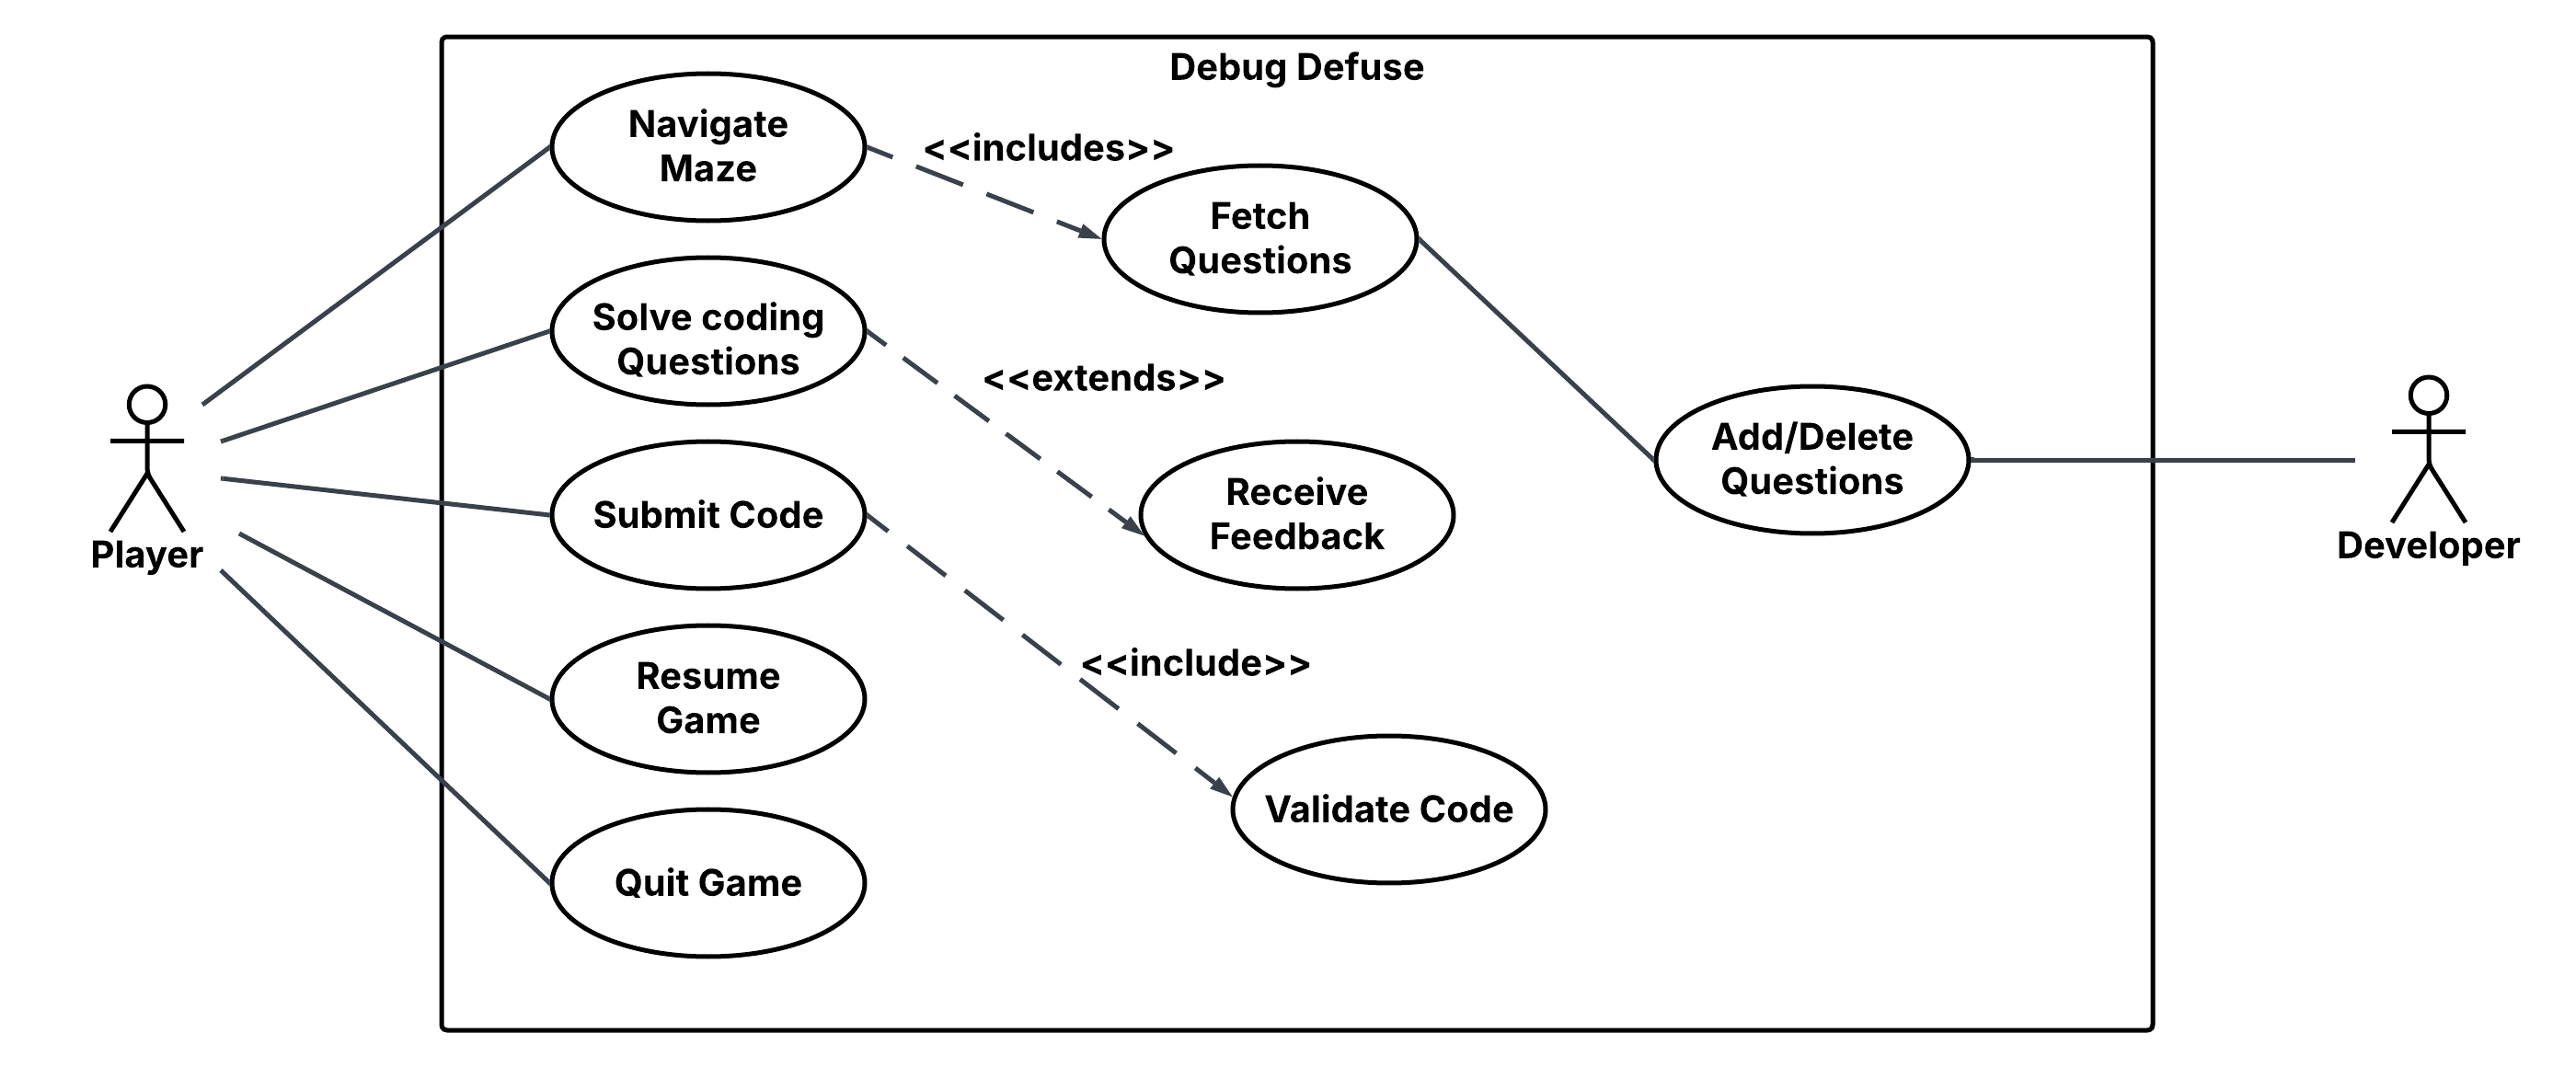
\includegraphics[width=1\textwidth,height=0.6\textwidth]{KV_use.png}
    \caption{Use case Diagram}
    \label{fig:Use_case}
\end{figure}
diagram explanation

 \section{Activity Diagram}
 \subsection{Character Movement}
\begin{figure}[H]
    \centering
    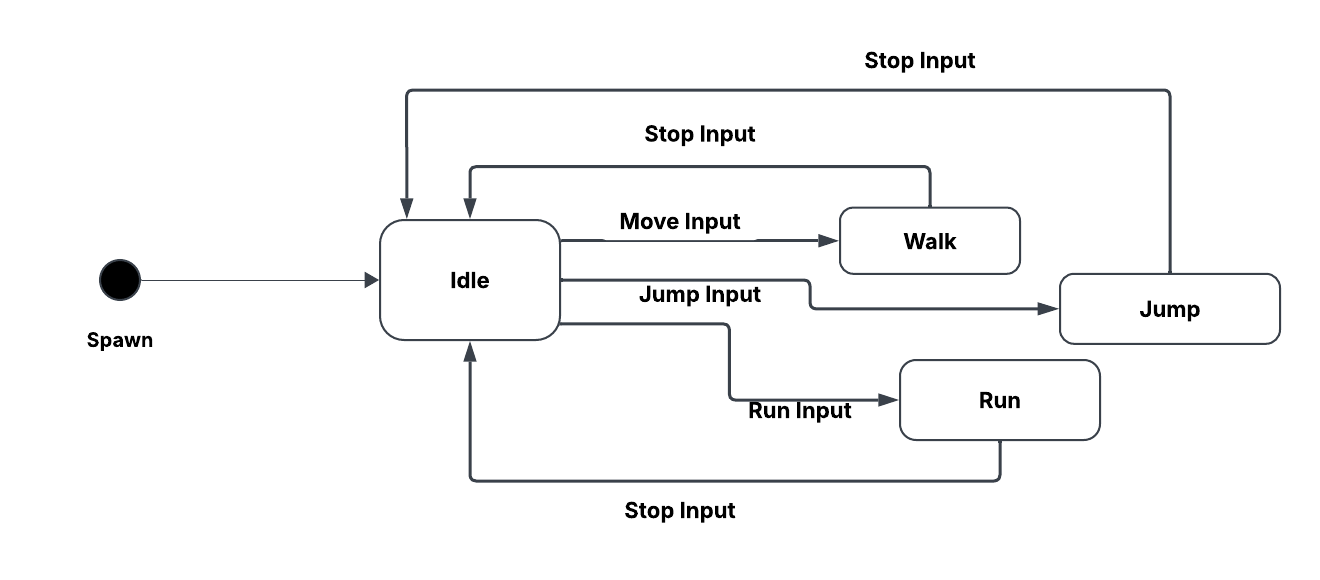
\includegraphics[width=1\textwidth,height=0.6\textwidth]{player_state.png}
    \caption{activity diagram}
    \label{fig:Use_case}
\end{figure}
diagram explanation
\subsection{Gameplay}
\begin{figure}[H]
    \centering
    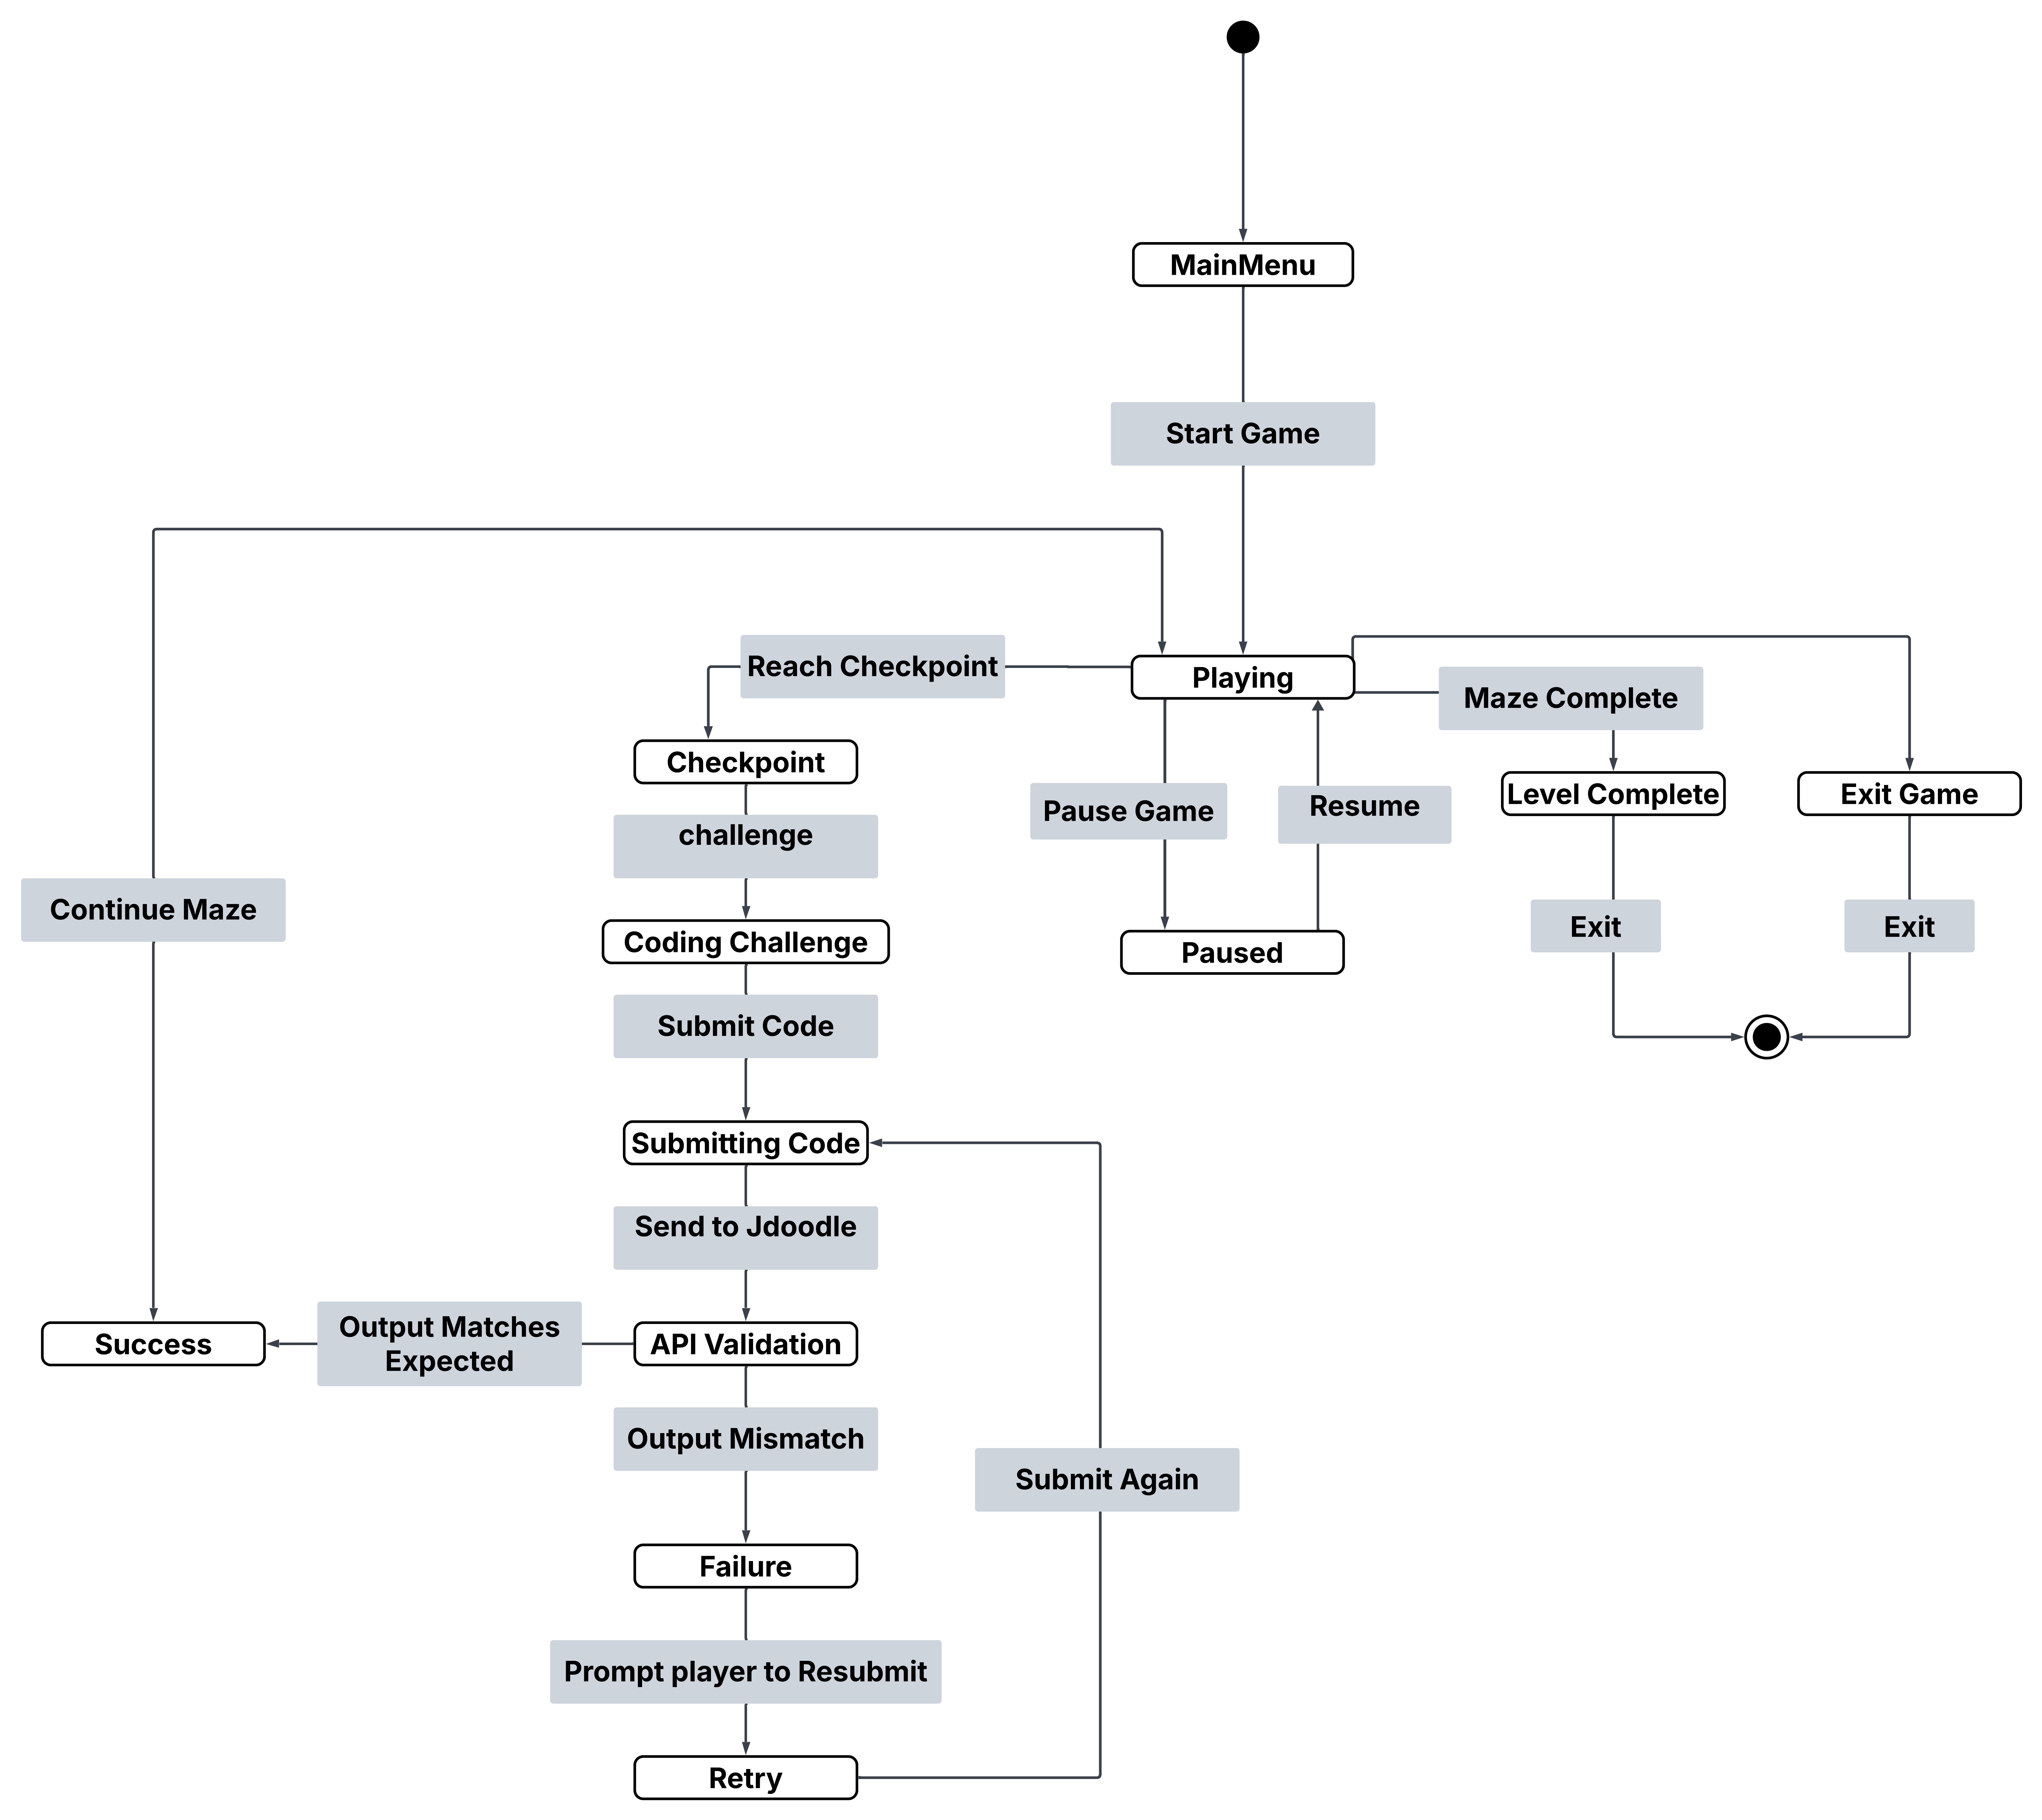
\includegraphics[width=1\textwidth]{game_chart (1).png}
    \caption{activity Diagram-Full Gameplay}
    \label{fig:Use_case}
\end{figure}
This State Chart diagram (Figure 4.3) represents the game flow of "Debug Defuse." It begins at the Main Menu, where the player can choose to Start Game, transitioning into the Playing state. During gameplay, the player will reach a Checkpoint that triggers a Coding Challenge. Upon submitting the code, it is sent to JDoodle for API Validation. If the output matches the expected result, the player can Continue Maze toward Success. In case of a mismatch, the player is prompted to Resubmit the code until successful. The player can also Pause, Resume, or Exit the game at any time, and upon Maze Completion, the level is marked complete and leads to exiting the game.
 \section{project Design}
 Game design is the process of creating the rules, mechanics, story, and overall structure of a game to provide an engaging and interactive experience for players. It involves designing gameplay elements such as levels, objectives, challenges, characters, and user interfaces to ensure a balanced and enjoyable experience. Good game design focuses on player engagement, progression, and feedback, making sure the game is both fun and challenging. It also includes aspects like storytelling, visual aesthetics, and sound design to create an immersive world.\\\\
 In Debug Defuse, the game design focuses on integrating coding challenges into an interactive 3D maze environment. Players navigate the maze, solving programming problems at checkpoints to progress. The design balances gameplay and learning by incorporating real-time code validation, user-friendly UI elements, and engaging visual effects. 
 educational and immersive.

 \subsection{UI Design}
\textbf{contents and images of your project's UI Design}

\subsection{Player Design}
\medskip
The player design in Debug Defuse is carefully crafted to ensure an engaging and immersive gaming experience. The character is designed to be visually appealing and functionally responsive, making it enjoyable to control within the game’s 3D maze environment.\\\\
\noindent
To achieve high-quality animations and realistic movement, the character model was sourced from Mixamo, a widely used platform that provides pre-rigged 3D character models with smooth, natural-looking animations. This choice ensures that the player has fluid animations for movement, jumping, and interactions with the game environment, enhancing the overall realism of the game.\\\\
\noindent
The movement mechanics are designed to be precise and responsive, allowing players to navigate through the maze smoothly. Whether walking, running, or jumping, the controls respond instantly to user input, ensuring a seamless gameplay experience. This level of responsiveness is crucial, especially in a game that requires precision in movement, as players must reach specific checkpoints and interact with coding challenges effectively.\\\\  
\noindent
To make the character feel more alive and interactive, different animations such as idle, walking, running, and jumping states are integrated using Unity’s Animator System. The Animator System ensures seamless transitions between animations, preventing unnatural or abrupt movements. For instance, if the player stops moving, the character automatically shifts to an idle animation, making the experience more immersive.\\\\  
\noindent
Beyond just movement, the character is also designed to interact dynamically with the game’s environment. When reaching a checkpoint, the player character triggers coding challenges, initiating the problem-solving phase of the game. Additionally, the character’s interaction with obstacles, walls, and pathways is carefully programmed to prevent issues like clipping through walls or unintended glitches.\\\\  
\noindent
By combining high-quality Mixamo animations, Unity’s Animator System, precise movement mechanics, and interactive elements, the player character in Debug Defuse offers a realistic, engaging, and smooth gameplay experience, making the game both educational and enjoyable for players.
\\\\
\begin{figure}[H]
    \centering
    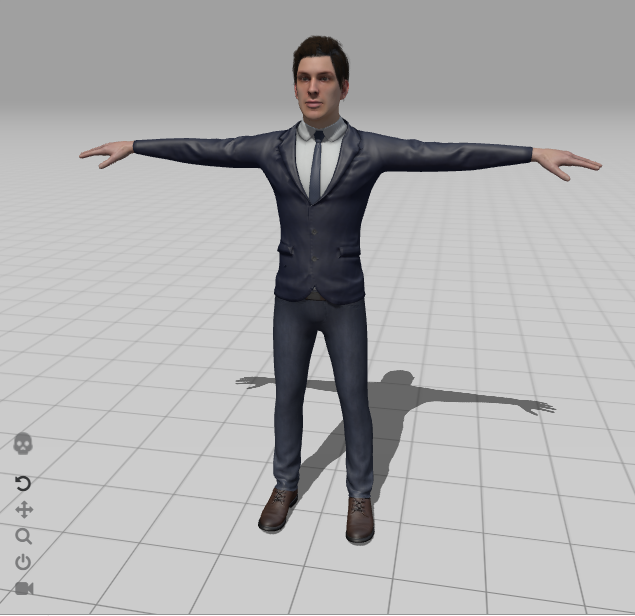
\includegraphics[width=0.5\textwidth]{joe.png}
    \caption{Charcter from mixamo}
    \label{fig:Use_case}
\end{figure}
\begin{figure}[H]
    \centering
    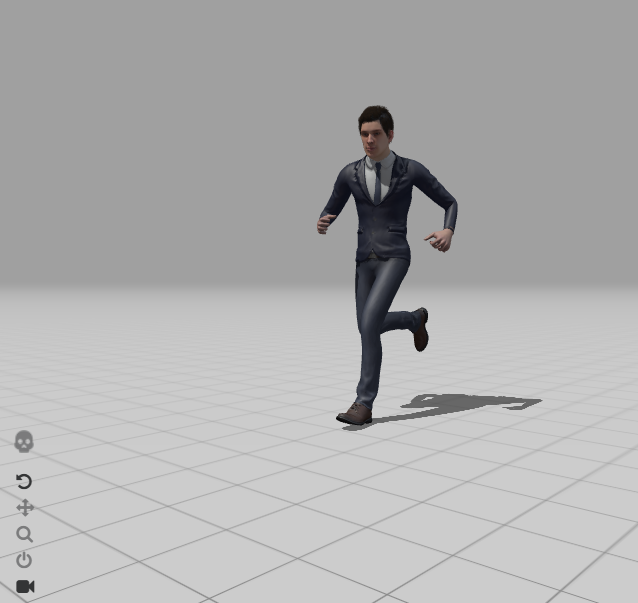
\includegraphics[width=0.7\textwidth]{joe_run.png}
    \caption{Character Run}
    \label{fig:Use_case}
\end{figure}
\noindent
Character in this Figure 4.16 can be directed using  four directional arrows/ASWD keys  to move the character in different directions, and the shift key is used for the character to sprint.
\begin{figure}[H]
    \centering
    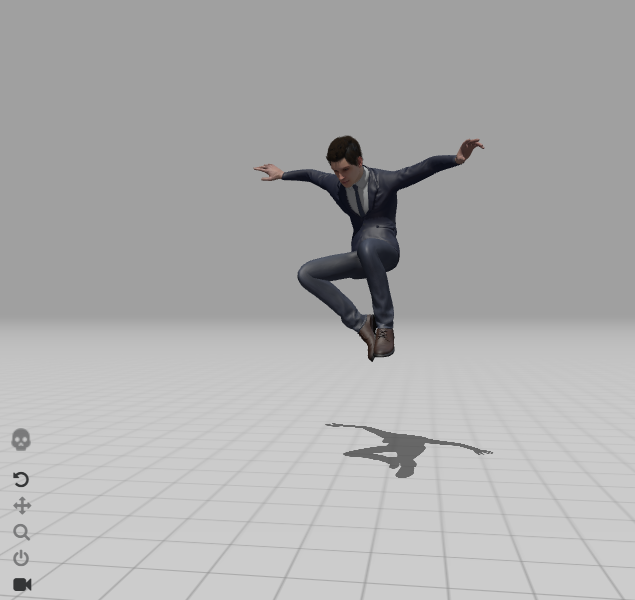
\includegraphics[width=0.6\textwidth]{joe_jump.png}
    \caption{Character jump}
    \label{fig:Use_case}
\end{figure}
\noindent
Figure 4.17 illustrates the player’s jump animation triggered by pressing the space bar. Since gravity is already applied to the player, they naturally return to the ground after the jump. We can set the jump amount which
determines how much air time the player gets.
\subsection{Background Score Design}
Background score in games plays a vital role in enhancing the overall player experience. It sets the mood, builds tension, and provides emotional depth to different game scenarios. Whether it’s an action-packed sequence, a calm exploration phase, or a suspenseful moment, the background music helps immerse the player in the virtual world, making gameplay more engaging and memorable.\\\\
Ableton Live is a professional digital audio workstation (DAW) widely used for music production, sound design, and live performances. In the development of Debug Defuse, Ableton Live was utilized to compose and produce custom background music that enhances the overall gaming experience. A intense and immersive score was created for the main menu to set a welcoming tone, while a more calm and ambient soundtrack was designed for in-game exploration and coding challenges. Using Ableton’s powerful tools like MIDI sequencing, audio effects, and virtual instruments, the background score was tailored to match the mood and pacing of different gameplay sections, providing players with an engaging and atmospheric audio experience.
\subsection{Sound Effects}
Sound effects play a crucial role in enhancing the realism and immersion of a game. In Debug Defuse, character sound effects such as footsteps, jumps, and landings were sourced and synchronized using Mixamo’s animation system. These effects were integrated into the Unity project to align with the character’s actions, making movements feel more natural and responsive. Each animation trigger is paired with a corresponding audio cue, helping players feel more connected to the environment. This use of sound effects not only adds depth to gameplay but also improves user engagement by providing auditory feedback that complements the visual and interactive elements of the game.
\subsection{Question Design}
The Questions are stored in JSON format which helps the system to easily and  randomly fetch the questions from file. Each question is displayed at specific checkpoints within the maze, requiring players to submit a correct solution before progressing further. Real-time validation using the JDoodle API provides immediate feedback, helping players understand errors and improve their coding skills. This interactive approach makes learning programming both fun and challenging.\\\\
\textbf{JSON File Structure}\\\\
The JSON file in my project stores coding questions in a structured format, making it easy to retrieve and display them in the game. Each question is represented as an object in a list, containing key attributes such as \texttt{questionType}, \texttt{questionText}, \texttt{description}, \texttt{input},and\\
\texttt{expectedOutput}. 
\\\\
In the game, when a player reaches a checkpoint, the system fetches a question from this JSON file based on predefined logic. The \texttt{questionText} presents the problem statement, and `description` provides additional details. The \texttt{input} field gives a sample input that the player’s code needs to process, while \texttt{expectedOutput} serves as a reference to verify the correctness of the submission. This structure ensures seamless integration with the JDoodle API, which compiles and executes the player’s code, comparing its output against \texttt{expectedOutput}. By using JSON, the game efficiently manages and updates coding challenges, enhancing flexibility and scalability.

\begin{lstlisting}[style=csharpstyle]
[
    {
        "questionType": "Coding",
        "questionText": "Reverse a string",
        "description": "Given a string, reverse the string and return it.",
        "input": "hello",
        "expectedOutput": "olleh"
    },
    {
        "questionType": "Coding",
        "questionText": "Find the factorial of a number",
        "description": "Write a function to compute the factorial of a given number 'n'.",
        "input": "5",
        "expectedOutput": "120"
    },
    {
        "questionType": "Coding",
        "questionText": "Palindrome check",
        "description": "Given a string, check if it is a palindrome.",
        "input": "madam",
        "expectedOutput": "true"
    },
    {
        "questionType": "Coding",
        "questionText": "Find the missing number in an array",
        "description": "Given an array containing 'n' distinct numbers taken from 1 to 'n+1', find the missing number.",
        "input": "[1, 2, 3, 5, 6]",
        "expectedOutput": "4"
    },
]
\end{lstlisting}



